% ------------------------------------------------------------------------------
% Chapter 3
% ------------------------------------------------------------------------------
\chapter{Research Methodology} % enter the name of the chapter here
\label{cha:ch3_methodology} % enter the chapter label here (for cross referencing)

\section{Introduction}
\label{sec:Introduction}
This chapter presents and justifies the methodological approach adopted to examine the influence of organisational culture and leadership on the return on investment (ROI) realised from AI coding assistants in software engineering teams. Given the complexity of the constructs under investigation, organisational culture, leadership, the assimilation quality of AI coding assistants, and ROI, it was essential that the research design be methodologically sound, so as to support the validity and generalisability of the findings. \textcite{Creswell2018} argues that the research design adopted should align closely with the research question(s) and the underlying theoretical framework. As this study sought to test relationships between constructs, to assess a mediating effect, and to do so while accounting for the measurement structure of each construct, a quantitative design combining preliminary correlational analysis with partial least squares structural equation modelling (PLS-SEM) was adopted. The chapter proceeds by outlining the research philosophy, research design, research hypotheses, population and sampling strategy, measurement and operationalisation of constructs, data collection procedure, data analysis techniques, research limitations, and the ethical considerations that guided the research.

\section{Research Philosophy}
\label{sec:Research Philosophy}
This paper is based on a post-positivist epistemology, which posits that social phenomena can be studied in a systematic manner, although measurement can never be perfect \autocite{Creswell2018}.

\subsection{Suitability of Post-Positivism for This Study}
\label{sec:Suitability of Post-Positivism for This Study}
The hypothesis testing process measures to what extent the relationships described in the conceptual framework are valid based on data. In quantitative analysis, hypotheses originate from theoretical frameworks presented in literature and are compared with empirical information. Consequently, researchers can determine whether or not links exist between different factors including organisational culture, leadership, the introduction of artificial intelligence, and profitability. Hypothesis testing is one of the key processes in quantitative investigations because it enables examining the above-mentioned theoretical frameworks and identifying whether or not the data support the proposed dependent and independent variables \autocite{Creswell2018}.

\begin{itemize}
	\item \textbf{Testing hypothesised relationships}
\end{itemize}
When testing relationships between concepts, one must verify the relationships indicated in the conceptual scheme against empirical data. In quantitative research, hypotheses are usually derived from the structure theories provided by literature. Thus, in quantitative studies, the researcher can state whether any relationships exist between such variables as organisational culture, leadership style, AI adoption, or ROI, etc. Hypothesis testing in quantitative research is of utmost importance since it allows testing theoretical schemes \autocite{Creswell2018}.

\begin{itemize}
	\item \textbf{Measuring latent variables}
\end{itemize}
Latent constructs are abstract concepts that cannot be measured directly, although they can be assessed through multiple indicators. In this study, organisational culture, leadership, and the assimilation quality of AI coding assistants were treated as latent constructs, as each represents complex organisational behaviour rather than a directly observable variable. Such constructs were measured through structured survey items and scales that had previously been validated for this purpose, and their measurement properties, indicator loadings, internal consistency, and convergent validity, were formally assessed as part of the structural equation model described in Section~\ref{sec:Data Analysis} \autocite{Hair2019}.

\begin{itemize}
	\item \textbf{Estimating relationships between variables}
\end{itemize}
Estimating the relationships proposed by a theoretical framework requires an assessment of both the direct associations between variables and any indirect pathways through which one variable influences another. In this study, the relationships of interest describe the association of organisational culture and leadership with the ROI realised from AI coding assistants, and the extent to which this association operates through the quality with which the tools are assimilated into software engineering practice. Pearson correlation analysis was used as a preliminary, descriptive screening step, after which partial least squares structural equation modelling was used as the confirmatory analysis to estimate the measurement model, the structural paths, and the specific indirect (mediated) effects among these constructs \autocite{Hair2019}.

\begin{itemize}
	\item \textbf{Generating generalisable findings}
\end{itemize}
One of the main goals of quantitative research is to come up with results that can be generalised beyond the specific research sample. By obtaining a sufficiently large sample of software engineers, this paper aimed to generalise its results to reflect a wider population of organisations. Therefore, the application of statistical techniques, such as bootstrapped significance testing made it possible to assess the degree of probability that the association being studied is real rather than a matter of chance thus providing evidence to organisation and scholarly community alike \autocite{Bryman2016}.

The employment of structured surveys and objective significance testing is in line with the post-positivist method of research \autocite{Hair2019}.

\section{Research Design}
\label{sec:Research Design}
\subsection{Quantitative Correlational and Structural Design}
\label{sec:Quantitative Correlational and Structural Design}
The study employed a cross-sectional quantitative design, combining a preliminary correlational stage with partial least squares structural equation modelling (PLS-SEM), to test the hypothesised relationships between organisational culture, AI leadership and governance support, the assimilation quality of AI coding assistants, and ROI.

Quantitative research techniques help to study relationships between variables \autocite{Bryman2016}. The reason for using PLS-SEM analysis is that it deals with the model including a mediating variable, several latent variables that are reflectively measured, and several observed covariates, as well as its low requirements for distribution limits \autocite{Hair2019}. The analysis was carried out in line with PLS-SEM standards and was completed in two phases. The first phase was to find descriptive statistics, reliability, and Pearson coefficient for the data. The second stage dealt with constructing a reflective type measurement model and structural models, which helped to provide estimates of the loadings of indicators, verify internal consistency, perform statistical analysis of the model including validity of discriminant and convergent types and coefficients of structural paths \autocite{Hair2019}. Still, it is important to understand the difference between two phases, since a big correlation value between the independent variable and ROI can be treated as a hypothesis just through taking into account the variance, mediating path and control variables used in the last modeling stage.

The structural model specified organisational culture and AI leadership and governance support as exogenous predictors of assimilation quality, assimilation quality as a mediating construct, and ROI as the dependent construct. Organisational readiness, team size, developer experience, and adoption duration were entered as control variables with direct paths to ROI, so that the core theoretical relationships could be assessed net of these contextual factors (Section~\ref{sec:Control Variables}).

\section{Research Hypotheses}
\label{sec:Research Hypotheses}
Consistent with the conceptual framework and the post-positivist emphasis on testing hypothesised relationships, the following hypotheses were formulated to guide the analysis:

\begin{itemize}
	\item[\textbf{H1:}] Organisational culture has a significant positive relationship with the ROI realised from AI coding assistants.
	\item[\textbf{H2:}] AI leadership and governance support has a significant positive relationship with the ROI realised from AI coding assistants.
	\item[\textbf{H3:}] The assimilation quality of AI coding assistants has a significant positive relationship with the ROI realised from AI coding assistants.
	\item[\textbf{H4:}] The assimilation quality of AI coding assistants mediates the relationship between (a) organisational culture and (b) AI leadership and governance support, and the ROI realised from AI coding assistants.
\end{itemize}

These hypotheses reflect the study's central proposition that organisational culture and leadership are associated with the ROI realised from AI coding assistants, and that this association operates, in whole or in part, through how well the tools are assimilated into software engineering practice. Because H1 and H2 concern the overall association between each predictor and ROI, they were evaluated using the total effect estimated by the structural model (the sum of each predictor's direct effect on ROI and its indirect effect through assimilation quality), consistent with the mediation-testing logic set out in Section~\ref{sec:Data Analysis}; the direct and indirect components of this total effect were then examined separately to test H4. Organisational readiness, team size, developer experience, and adoption duration were entered into the structural model as control variables with direct paths to ROI (Section~\ref{sec:Control Variables}); consistent with their role as controls rather than as theorised predictors, no directional hypotheses were formulated for these paths. Figure~\ref{fig:hypothesised_model} presents the hypothesised model diagrammatically.

%\begin{figure}[htbp]
%	\centering
%	\resizebox{\linewidth}{!}{%
%		\begin{tikzpicture}[
%			construct/.style={draw, rounded corners=8pt, align=center, minimum width=2.8cm, minimum height=1.1cm, font=\small},
%			every node/.style={font=\small}
%			]
%			\node[construct] (OC) at (0,2.2) {Organisational\\Culture};
%			\node[construct] (LP) at (0,0) {AI Leadership and\\Governance Support};
%			\node[construct] (AQ) at (4.8,1.1) {Assimilation Quality of\\AI Coding Assistants};
%			\node[construct] (ROI) at (9.6,1.1) {Return on\\Investment (ROI)};
%			\node[construct, minimum width=4.2cm] (CTRL) at (9.6,-1.8) {Controls: Organisational Readiness,\\Team Size, Developer Experience,\\Adoption Duration};
			
%			\draw[->, thick] (OC) -- (AQ) node[midway, above, sloped] {H1};
%			\draw[->, thick] (LP) -- (AQ) node[midway, below, sloped] {H2};
%			\draw[->, thick] (AQ) -- (ROI) node[midway, above] {H3};
%			\draw[->, thick] (CTRL) -- (ROI);
%		\end{tikzpicture}%
%	}
%	\caption{Hypothesised model. Assimilation quality is hypothesised to mediate the relationship between organisational culture and AI leadership and governance support, and the ROI realised from AI coding assistants (H4). Organisational readiness, team size, developer experience, and adoption duration were entered as control variables with direct paths to ROI.}
%	\label{fig:hypothesised_model}
%\end{figure}

% ------------------------------------------------------------------------------
% Hypothesised_structural_model image
% ------------------------------------------------------------------------------
\begin{figure}[H]
	\begin{center}
		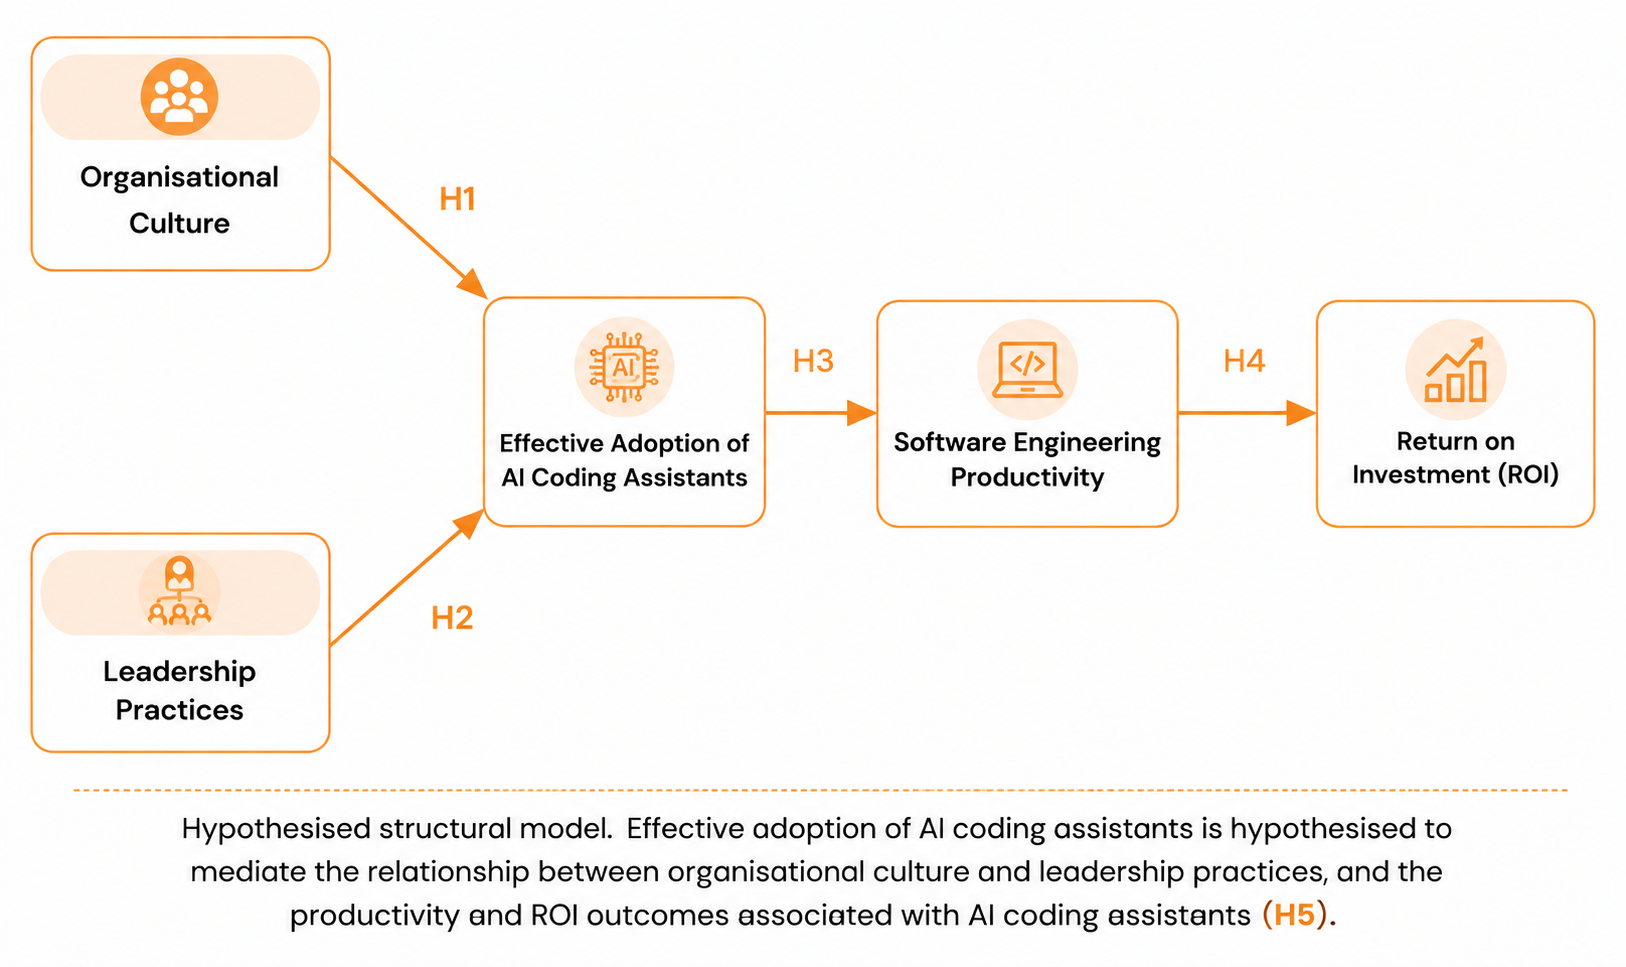
\includegraphics[width = 1\textwidth]{Images/Hypothesised_structural_model} % enter the filename here
		\caption{hypothesised model} % enter the figure caption here
		\label{fig:hypothesised_model} % enter the figure label here (for cross referencing)
	\end{center}
\end{figure}

Hypothesised model. Assimilation quality is hypothesised to mediate the relationship between organisational culture and AI leadership and governance support, and the ROI realised from AI coding assistants (H4). Organisational readiness, team size, developer experience, and adoption duration were entered as control variables with direct paths to ROI.

\section{Population and Sampling}
\label{sec:Population and Sampling}
\subsection{Target Population}
\label{sec:Target Population}
The study focused on software engineering teams within large organisations in South Africa that uses AI coding assistants.

\subsection{Sampling Strategy}
\label{sec:Sampling Strategy}
A purposive sampling strategy was adopted on this study, focusing on organisations that met the following criteria:
\begin{itemize}
	\item Used AI coding assistants;
	\item Had used AI coding assistants for at least six months; and
	\item Maintained measurable software engineering metrics.
\end{itemize}

The participants of the study comprised of software engineering professionals who worked in these organisations including developers, technical leads, and engineering managers, and who were selected using stratified sampling technique. 

Following the requirement of the methodological guidance, which states that there should be at least 200 in order to conduct correlation/SEM analysis for obtaining reliable and valid estimates \autocite{Hair2019}, the target sample size of this study was 250 to 300 participants. There were a total of 357 responses received, out of which 355 responses fulfilled the eligibility criteria of currently using AI coding assistants.

This minimum was corroborated after data collection using two established PLS-SEM sample-size heuristics, applied to the final analytical sample ($N=354$) and the largest number of predictors entered on a single construct in the structural model (seven, for ROI). The ten-times rule, which recommends at least ten observations per predictor on the most heavily predicted construct, implies a minimum of 70; the more formal inverse-square-root method \autocite{Kock2018}, which relates minimum sample size to the smallest structural path coefficient a study should be powered to detect at 5\% significance and 80\% power, implies a minimum of 275 to reliably detect a path as small as .15, and of 99 to detect a path as small as .25. The final analytical sample of 354 therefore exceeded both the ten-times-rule minimum and the inverse-square-root minimum for every path coefficient found to be statistically significant in Chapter Four (all of which exceeded .35 in magnitude), though it fell short of the inverse-square-root minimum needed to reliably detect a path as small as .12 (which would require $N=430$). Several of the non-significant control-variable paths reported in Chapter Four were smaller than this study was well powered to detect, so their non-significance should be read as inconclusive rather than as confident evidence of a true null effect.

\section{Measurement and Operationalisation}
\label{sec:Measurement and Operationalisation}
For each latent construct, measurement scales were created to ensure the construct validity \autocite{DeVellis2022}. A five-point Likert scale was used to measure each construct. As per the numeric coding system agreed for this analysis, responses were coded as 1 (Strongly Agree), 2 (Agree), 3 (Neither Agree nor Disagree), 4 (Disagree), and 5 (Strongly Disagree); for all items, the same direction was used, where a lower mean score means a stronger agreement. There is no influence of this coding option on the substantive conclusions obtained from the analysis; the reliability coefficients remain unaffected due to the uniform use of recording and the correlation or path coefficient of having two constructs coded in the same way showcases the same sign; it is stressed in this section and in chapter four as well to clarify the interpretation of means and skewness statistics.

\subsection{Organisational Culture}
\label{sec:Organisational Culture}
\textbf{Organisational culture} was assessed using adapted and validated scales addressing the following dimensions:

\begin{itemize}
	\item \textbf{Psychological Safety}
\end{itemize}
\textbf{Psychological safety} refers to the degree of comfort felt by members of a group to experiment, question, and contribute ideas without fear of criticism. In software engineering teams using AI coding assistants such as GitHub Copilot, psychological safety enables developers to question the suggestions generated by the tool. Developers who feel safe experimenting with the tool are better placed to become proficient in its use and to draw effectively on generative AI. Literature on the use of generative AI in knowledge work indicates that productivity gains are more pronounced where workers engage with such tools collaboratively \autocite{Noy2023}.

\begin{itemize}
	\item \textbf{Learning Orientation}
\end{itemize}
The \textbf{learning orientation} refers to how much the organisation values continual learning and development of skills. In an organisation that is implementing generative AI tools, the members will need to develop the necessary skills to work with these technologies effectively. Thus, organisations that have a strong learning orientation possess a higher chance to be able to implement generative AI successfully. Empirical studies show that generative AI has a high potential to increase productivity at work due to its application by employees' on their jobs \autocite{Brynjolfsson2025}.

\begin{itemize}
	\item \textbf{Knowledge Sharing}
\end{itemize}
\textbf{Knowledge Sharing} refers to the transfer of knowledge and skills among the members of a team. In teams utilising AI coding assistants, this generally involves the transfer of knowledge related to prompts, methods of debugging and best practices for applying the tool, which in turn allows the team to take advantage of generative AI. Empirical studies show that software development teams depend on such knowledge sharing to use the tools wisely \autocite{Sergeyuk2025}.

\begin{itemize}
	\item \textbf{Digital Openness}
\end{itemize}
\textbf{Digital openness} refers to the willingness of organisations and their people to accept new digital technologies. Organisations that display digital openness are more likely to accept generative AI tools and to adapt their processes accordingly. In software engineering, digital openness is likely to encourage the adoption of AI coding assistants and to support developers in exploring new ways of improving their productivity.

The organisational culture scale comprised seven items covering experimentation, knowledge sharing, learning orientation, collaboration, innovation support, responsible use, and the evaluation of measurable value, and was measured using the five-point Likert scale described above \autocite{Bryman2016}.

\subsection{AI Leadership and Governance Support}
\label{sec:AI Leadership and Governance Support}
AI leadership and governance support was assessed using a four-item scale covering the following dimensions:

\begin{itemize}
	\item \textbf{Executive Sponsorship}
\end{itemize}
\textbf{Executive sponsorship} refers to the degree to which leaders of the organisation advocate for the use of generative AIs and make it clear how they should be used in the development. When the top leaders show their support for AI programming assistants, it provides assurance to the employees' that this technology is of importance and meets the expectations of the organisation. Research in the field of the use of generative AI in complex processes has shown that workers feel more confident in using AI technologies with support from the organisation \autocite{Noy2023}. Research on the phenomenon of the use of AI has shown that executive sponsorship allows for the orderly adoption of new technologies across departments \autocite{Brynjolfsson2025}.

\begin{itemize}
	\item \textbf{Metric Alignment}
\end{itemize}
In this context, \textbf{metric alignment} is defined as the degree to which business leaders express the expected value that will come from using an AI coding assistant, in order to ensure that the performance expectations meet the objectives set before AI adoption. Studies on generative AI productivity show that organisational outcomes are realised only if performance indicators match AI usage efficiency and task accomplishment. The alignment of metrics involves business leaders indicating the expected benefits from the use of an AI coding assistant and simultaneously managing performance expectations in light of these benefits \autocite{Noy2023}.

\begin{itemize}
	\item \textbf{Resource Support}
\end{itemize}
\textbf{Resource support} is defined as the funding, know-how, and labour that must be allocated for successful implementation of AI solutions. For instance, the successful use of AI coding assistants requires investment in training developers, integration into software development environments as well as in infrastructure and constant analysis of the results of AI coding assistants' implementation. \textcite{Babina2024} states that companies would not benefit from using such tools without enough resource support.

\begin{itemize}
	\item \textbf{Governance Clarity}
\end{itemize}
\textbf{Governance clarity} refers to the extent to which leaders ensure that governance, risk, and quality concerns related to AI coding assistants are actively addressed. Generative AI tools such as Copilot carry significant governance implications for intellectual property, security, and software quality assurance, and organisations therefore need well-defined governance structures to frame the use of AI-generated code and to establish clear accountability. Research on AI governance has found that organisations with well-defined structures are better placed to manage technology risk while still realising the associated productivity benefits \autocite{Hradecky2022}.

\subsection{Assimilation Quality of AI Coding Assistants}
\label{sec:Assimilation Quality of AI Coding Assistants}
The quality of assimilation refers to the level to which coding assistants are integrated in the activities of a software engineer in a productive way as opposed to simply being installed. In this regard this concept encompasses how well the instruments are incorporated into daily workflow, the regularity of the usage, the extent to which AI-produced output is scrutinised and the degree to which the usage of the technology is in compliance with governance and quality assurance standards. Some empirical studies related to coding assistants reveal that they can boost developers productivity, although the magnitude of productivity increase depends on the degree of technology integration into the processes \autocite{Brynjolfsson2025}. The construct under discussion is based on the eight-item measure that addresses the following aspects:

\begin{itemize}
	\item \textbf{Workflow Integration}
\end{itemize}
\textbf{Workflow integration} relates to how AI coding assistants are incorporated into the existing development workflow and how they are integrated into collaboration efforts, like code review, testing, and documentation. The tools that are integrated into the existing workflow are most likely to be welcomed by developers. Research has found that using AI within established workflows leads to productivity gains compared to its disruptive nature \autocite{Brynjolfsson2025}.

\begin{itemize}
	\item \textbf{Usage Consistency}
\end{itemize}
\textbf{Usage consistency} means to what extent AI coding assistants are used in accordance with certain expectations and standards during the software creation process by the given team. Studies show that any form of generative AI will lead to better productivity results in the case of its consistent application \autocite{Noy2023}.

\begin{itemize}
	\item \textbf{Trust Calibration}
\end{itemize}
\textbf{Trust calibration} is the developers capacity to correctly trust AI-generated outputs. This is reflected in the extent of evaluation of AI-generated code suggestions during their previous review before using them in the development process. Studies on how human beings and AI interact have revealed that success largely depends on the ability to find this very balance \autocite{Noy2023}.

\begin{itemize}
	\item \textbf{Training and Governance Support}
\end{itemize}
The indicator refers to whether the developers have received sufficient training on using AI programming assistants successfully, as well as whether there is proper governance and quality control of using AI-powered functions on the site. AI programming has shown that deeper engagement with the usage of AI technology positively affects the efficiency of development and problem-solving \autocite{Brynjolfsson2025}.

\subsection{Return on Investment (ROI)}
\label{sec:Return on Investment Measurement}
ROI was operationalised as the perceived business value realised from AI coding assistants, following the perceptual approach to ROI measurement common in information systems research where direct financial data are not accessible to individual respondents \autocite{Hair2019}. A 15-item scale assessed ROI across three conceptual levels:

\begin{itemize}
	\item \textbf{Task-Level ROI}
\end{itemize}
Task-level ROI (five items) captures the extent to which AI coding assistants have improved individual developer productivity, reduced the time required to complete coding tasks, improved the efficiency of routine development tasks, contributed to improved software quality, and improved overall delivery performance at the level of individual work.

\begin{itemize}
	\item \textbf{Workflow-Level ROI}
\end{itemize}
Workflow-level ROI (four items) captures the extent to which AI coding assistants have improved the efficiency of the overall development workflow, contributed to improved software quality, reduced rework, and improved delivery performance at the level of the team's workflow.

\begin{itemize}
	\item \textbf{Firm-Level ROI}
\end{itemize}
Firm-level ROI (six items) captures the extent to which AI coding assistants have contributed to lower software development costs, faster time to market, innovation in software products or services, benefits that outweigh the costs of adoption, business value beyond individual coding tasks, and financial value that justifies the investment made.

Because the three ROI levels are conceptually related facets of the same underlying construct, all 15 items were retained and were tested both as a single overall reflective construct and as three separate dimensional constructs; the two specifications were compared using the measurement evidence reported in Chapter Four (Section~\ref{sec:Discriminant validity}), and the final representation used in the structural model was selected on that basis, in line with the principle that model specification should follow theory and measurement evidence rather than the significance of any resulting path \autocite{Hair2019}.

\subsection{Control Variables}
\label{sec:Control Variables}
Four control variables were entered into the structural model with direct paths to ROI, so that the core theoretical relationships could be interpreted net of contextual influences that plausibly affect perceived ROI independently of organisational culture, leadership, or assimilation quality.

Organisational readiness was measured using a six-item scale assessing whether the organisation has the technical infrastructure to support AI coding assistants, whether developers have the necessary skills, whether the organisation is generally ready to adopt and integrate AI technologies, whether adequate governance mechanisms are in place, whether the organisation is prepared to address associated risks (security, privacy, intellectual property, and quality), and whether it has the capability to assess whether AI coding assistants are generating measurable value. Unlike the remaining three control variables, organisational readiness was modelled as a reflective latent construct measured by its six items.

Team size, developer experience, and adoption duration were each measured using a single categorical item from the survey's screening section (team size in bands from fewer than five to more than twenty developers; professional development experience in bands from less than two years to more than ten years; and adoption duration in bands from less than six months to more than two years) and were entered into the structural model as observed, single-indicator control variables. Team size and developer experience were retained as two distinct observed characteristics rather than combined into a single construct, since they describe conceptually different aspects of a respondent's context.

\section{Data Collection}
\label{sec:Data Collection}
Data were collected through a structured online questionnaire administered via Google Forms. Online questionnaires are widely used in organisational and information systems research owing to their effectiveness in reaching dispersed samples. The questionnaire comprised closed-ended items measured using the five-point Likert scale described in Section~\ref{sec:Measurement and Operationalisation}, assessing organisational culture, AI leadership and governance support, the assimilation quality of AI coding assistants, ROI, and organisational readiness, together with a short screening and demographic section covering AI coding assistant use, adoption duration, role, team size, and professional development experience.

The survey was shared through professional networks, IT societies, and tech forums. The participation was voluntary, and prior to data gathering ethical approval was secured. Survey participants who indicated no usage of an AI coding helper were eliminated from one of the important parts of the survey and filtered out in the eligibility part of the analysis (Chapter Four, Section~\ref{sec:Data Screening and Sample Profile}).

The questionnaire items were adapted from measurement scales validated in prior studies, an approach intended to support the reliability of the data collected.

Prior research on AI adoption suggests that the success of AI tools depends not only on the technology itself, but on how individuals and organisations adopt and use it \autocite{Brynjolfsson2025}. Accordingly, the study measured both behavioural and organisational dimensions of AI use.

\subsection{Pilot Testing}
\label{sec:Pilot Testing}
Before the full deployment of the questionnaire, a small group of software engineering practitioners took part in piloting the questionnaire, but they were not included in the sample used in the main study. In the pilot study, we assessed the clarity, length, and face validity of the items in the questionnaire, and adjusted the questionnaire accordingly before sending it to the target sample. Testing a questionnaire in this fashion is recommended so that measurement error can be minimized and it also make it easier for respondents to understand the questionnaire \autocite{DeVellis2022}.

\section{Data Analysis}
\label{sec:Data Analysis}
Data analysis proceeded in two stages, following established PLS-SEM practice for combining preliminary screening with confirmatory structural modelling \autocite{Hair2019}.

\textbf{Stage one: data screening and preliminary analysis.} The eligibility criterion (current use of an AI coding assistant) was applied first and independently of any subsequent result, yielding 355 eligible responses from 357 submitted; complete-case analysis was then applied to the eligible sample, yielding a final analytical sample of 354 (Chapter Four, Section~\ref{sec:Data Screening and Sample Profile}). Descriptive statistics (mean, standard deviation, minimum, maximum, skewness, and kurtosis) were computed for every item and for each construct, to characterise the sample and to check for out-of-range values and restricted variance. Internal consistency was assessed using Cronbach's alpha for each construct, computed separately for AI leadership and governance support, organisational culture, assimilation quality, organisational readiness, the 15-item ROI scale as a whole, and each of the three ROI dimensions individually, together with corrected item-total correlations. Common method bias was assessed using two procedures, Harman's single-factor test and a full-collinearity variance inflation factor test \autocite{Kock2015}, given that all constructs were measured by self-report from the same respondents at the same point in time. Finally, Pearson correlations were computed among provisional construct mean scores as a preliminary, descriptive view of the relationships between constructs; as noted in Section~\ref{sec:Quantitative Explanatory Design}, these correlations were not treated as the final test of the hypotheses.

\textbf{Stage two: PLS-SEM measurement and structural model.} A reflective measurement model was estimated for AI leadership and governance support, organisational culture, assimilation quality, ROI, and organisational readiness, together with a structural model specifying organisational culture and AI leadership and governance support as predictors of assimilation quality, assimilation quality and the four control variables (organisational readiness, team size, developer experience, and adoption duration) as predictors of ROI, and organisational culture and AI leadership and governance support as additional direct predictors of ROI. Measurement model quality was assessed using indicator outer loadings (retaining loadings at or above .708 as strong indicator contributions), Cronbach's alpha, composite reliability (Dillon-Goldstein's rho), average variance extracted (AVE, retaining constructs at or above .50), and the Dijkstra-Henseler consistency reliability coefficient (rho\textsubscript{A}), computed directly from the fitted model's outer weights and indicator correlation matrix using Dijkstra and Henseler's (2015) closed-form estimator \autocite{Dijkstra2015}, so that internal consistency was assessed using all three complementary coefficients rather than composite reliability and Cronbach's alpha alone. Discriminant validity was assessed using three procedures: the heterotrait-monotrait ratio of correlations (HTMT), with values below .85 treated as strong evidence of discriminant validity, values between .85 and .90 treated as borderline, and a percentile bootstrap 95\% confidence interval computed for every HTMT ratio so that discriminant validity could be assessed inferentially and not only against a fixed point-estimate threshold \autocite{Hair2019}; the Fornell-Larcker criterion, comparing the square root of each construct's AVE against its correlation with every other construct; and an inspection of item cross-loadings, checking that every indicator correlated most strongly with its own construct. Because the theoretical framework identifies ROI at three levels, HTMT evidence was used, together with a comparison of the model estimated with a single overall ROI construct against a model estimated with task-, workflow-, and firm-level ROI as three separate constructs, to select the final ROI specification reported in Chapter Four, consistent with the principle that this choice should be justified by measurement evidence rather than by whichever specification produces more significant paths \autocite{Hair2019}.

Structural model collinearity was assessed using the variance inflation factor (VIF), with values below 5 treated as free of serious multicollinearity. Structural path coefficients, their standard errors, t-values, and 95\% confidence intervals were estimated using bootstrapping (2,000 resamples, percentile method, two-tailed test), with a path treated as statistically supported where its 95\% confidence interval excluded zero. Effect sizes (f\textsuperscript{2}) were computed for each structural predictor by comparing the coefficient of determination (R\textsuperscript{2}) of the full model with that of a model omitting the predictor concerned, and R\textsuperscript{2} and adjusted R\textsuperscript{2} were reported for assimilation quality and ROI. The mediating effect of assimilation quality proposed in H4 was tested using the specific indirect effect (the product of the relevant path from organisational culture, or AI leadership and governance support, to assimilation quality, and the path from assimilation quality to ROI), with its own bootstrapped 95\% confidence interval; the pattern of direct and indirect results was then classified as indirect-only mediation, complementary partial mediation, competitive mediation, or no support for mediation, following standard PLS-SEM mediation-classification criteria \autocite{Hair2019}. Predictive relevance was assessed for each ROI indicator using a ten-fold cross-validated procedure in the spirit of PLSpredict, comparing the prediction error of the structural model with that of a linear regression benchmark and reporting Q\textsuperscript{2}\textsubscript{predict} for each indicator. Two robustness checks were performed: a comparison of the structural model estimated with and without the four control variables, and a comparison of the primary model with a sensitivity model excluding respondents who selected the most positive response option on every substantive item, together with the standardised root mean square residual (SRMR) as a supplementary approximate model-fit statistic. Finally, an importance-performance map analysis (IPMA) was conducted for the four constructs with a path to ROI, combining each construct's total effect on ROI (importance) with its rescaled mean score (performance), to translate the structural results into a managerial prioritisation \autocite{Hair2019}.

The PLS-SEM computations reported in Chapter Four were carried out using a Python-based implementation of the partial least squares path modelling algorithm, rather than the SmartPLS software package; this is stated explicitly here, since the two produce results based on the same underlying algorithm but are not the same software. Every statistic reported in Chapter Four that is defined by a published closed-form formula, including rho\textsubscript{A}, HTMT, the Fornell-Larcker criterion, and cross-loadings, was computed directly from that formula and is reported on the same basis as it would be in SmartPLS. Statistics that depend on random resampling, the structural path bootstrap and the specific indirect effect bootstrap, will vary slightly between any two runs of either toolchain unless the same random seed is fixed in both; this is a general property of bootstrapping rather than a limitation specific to the toolchain used here, and is noted so that the precise decimal values reported in Chapter Four are not mistaken for exactly reproducible constants.

Collectively, this analytical strategy was designed to generate empirical evidence on how organisational culture and AI leadership and governance support are associated with the ROI realised from AI coding assistants, the extent to which this association is explained by how well the tools are assimilated into software engineering practice, and how robust these relationships are once organisational readiness, team size, developer experience, and adoption duration are accounted for.

\section{Research Limitations}
\label{sec:Research Limitations}
As with any study, several methodological limitations should be acknowledged. First, the cross-sectional design captured relationships among variables at a single point in time; correlation, structural path, and mediation analysis can establish the strength, direction, and statistical significance of an association, but cannot establish causality with the same confidence as a longitudinal or experimental design \autocite{Creswell2018}. Second, all constructs were measured using self-reported items completed by the same respondents, which introduces the possibility of common method bias and social desirability bias; this risk is assessed directly in Chapter Four using Harman's single-factor test, and is compounded by a pronounced ceiling effect in the responses (Chapter Four, Section~\ref{sec:Data Screening and Descriptive Statistics}), which a sensitivity analysis excluding the most extreme response pattern shows materially affects the size, though not the direction, of some structural estimates. Third, organisational culture and AI leadership and governance support were found to be empirically difficult to separate on the more stringent HTMT criterion, including on that criterion's own bootstrap confidence interval, although not on the more conservative Fornell-Larcker criterion (Chapter Four, Section~\ref{sec:Discriminant validity}); this limits the extent to which their independent, direct effects on ROI can be separated in the structural model, even though their combined association with ROI, operating through assimilation quality, is estimated with more precision. Fourth, the three ROI sub-scales (task-, workflow-, and firm-level) were found not to be empirically distinguishable from one another, which supported the decision to represent ROI as a single overall construct in the final structural model, but also means the study cannot speak to whether organisational culture, leadership, or assimilation quality relate differently to ROI at the task, workflow, or firm level. Fifth, the use of purposive and stratified sampling, while appropriate for reaching organisations meeting the study's inclusion criteria, limits the extent to which the findings can be generalised beyond large South African organisations with at least six months of experience using AI coding assistants; the achieved sample also included a broader range of software engineering roles than the developers and team leads originally targeted, which is addressed further in Chapter Four. Sixth, ROI was operationalised through perceptual indicators rather than direct financial data, which may not fully capture the financial return realised by participating organisations. Finally, the scope of the structural analysis itself was bounded in two specific ways, disclosed here as deliberate decisions rather than oversights: measurement invariance and a multigroup comparison across role or team size (MICOM and PLS-MGA) were not tested, although the achieved sample would support this as a natural extension; and unobserved heterogeneity, nonlinear effects, and endogeneity were not modelled, each being a legitimate, more advanced extension beyond the scope of a single master's-level study. These limitations are revisited in Chapter Five, alongside recommendations for future research.

\section{Ethical Considerations}
\label{sec:Ethical Considerations}
All ethical aspects were taken into account in this research. Participation in the survey was voluntary, and respondents were informed of the purpose of the research prior to completing the questionnaire. The participants were assured that their responses would be kept anonymous.

No details that could help in identifying the respondents were obtained. The results of this research were used solely for academic purposes and stored in a secure way according to ethical principles underlying social research.

\section{Summary}
\label{sec:Summary}
This chapter has presented the methodological approach adopted in the study. A quantitative design combining preliminary correlational screening with partial least squares structural equation modelling was used to investigate the relationships between organisational culture, AI leadership and governance support, the assimilation quality of AI coding assistants, and ROI, net of the influence of organisational readiness, team size, developer experience, and adoption duration. Data were collected through a structured online survey of software engineering practitioners, and statistical techniques, including reliability analysis, Pearson correlation, and a bootstrapped PLS-SEM measurement and structural model, were used to test the hypothesised relationships within the conceptual framework.

Through this methodology, the study sought to generate empirical evidence on the influence of organisational and leadership factors on the value realised from generative AI tools in software engineering. The following chapter presents the results of this analysis.

